% -----------------------------------------------------------------------------
% Resultados
% -----------------------------------------------------------------------------

\chapter{Análise e Discussão dos Resultados}

\section{Provisionamento de infraestrutura}
\label{sec:provisionamento}

\subsection{Configuração Inicial}

Foi utilizado para o setup inicial uma imagem customizada do Ubuntu Server 20.04, que se valia de uma configuração prévia automatizada por meio de \href{https://cloudinit.readthedocs.io/en/latest/}{cloud-init}. Isso possibilitou a execussão de todas as máquinas mantendo a uniformidade de configurações inicias de SSH, usuário e permissões de {sudo} em 2 horas, considerando que a execussão foi a partir de uma única unidade de \emph{pen-drive}. A melhor opção seria disponibilizar em uma unidade de rede comum as máquinas que pudessem ser acessadas durante o boot inicial.

Para assegurar um acesso seguro a rede do Winet foi selecionado um computador para servir como \emph{load balancer} em rede privada e \emph{bastion host} para acesso externo. Neste configuração local realizada foi instalação de um agente de tunelamento reverso de rede \href{https://ngrok.io}{ngrok} para expor a porta 22 em um endpoint com IP público, na qual uma comunicação SSH poderia ser estabelicida mediante a chave adequada. Essa configuração foi necessária para agilizar o desenvolvimento provisinamento de segurança, enquanto um usuário de VPN não foi provisionado, e como a solução é semelhante a um tunelamento reverso de pora, em um endpoint efêmero, as confgiurações de rede da UFMG não forma expostas e pouco risco foi acrescido. 


\begin{figure}[!ht]
    \centering
    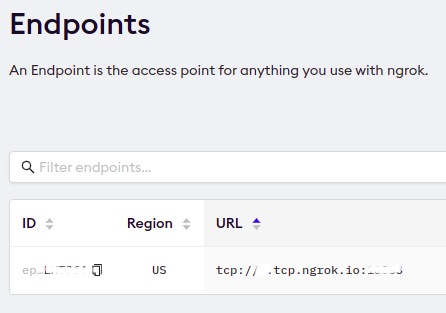
\includegraphics[width=0.5\textwidth]{04-figuras/ngrok.png}
    \caption{Ngrok Endpoint}
    \label{fig:ngrok}
\end{figure}

\begin{figure}[!ht]
    \centering
    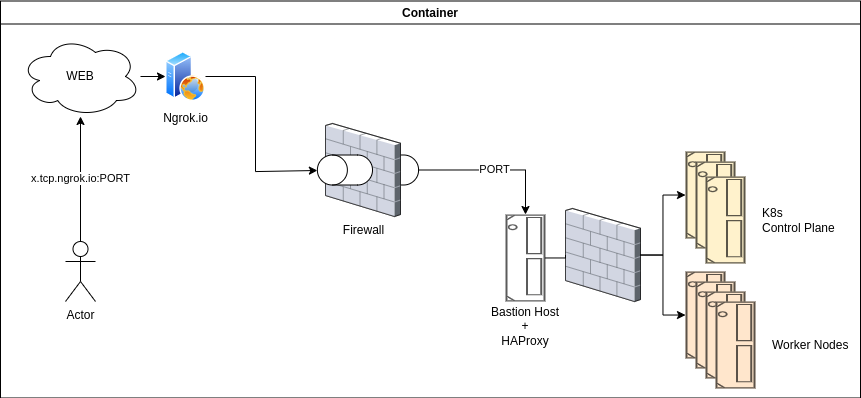
\includegraphics[width=0.8\textwidth]{04-figuras/ngroktcp.png}
    \caption{Ngrok Endpoint}
    \label{fig:ngroktcp}
\end{figure}

Juntamente a essa configuração foram realizados os seguintes configurações de segurança básicas:

\begin{itemize}
    \item instaladas fail2ban com throtlle 3 requisições falhas por minuto, limitando ataques \emph{brute-force} na porta SSH.
    \item foi desabilitado login root
    \item foi desabilitada login por com senha
    \item habilitado trafego na porta 22 de qualquer IP
    \item habilitado trafefo em qualquer porta de IPs dentro da faixa de CIDR da subnet
\end{itemize}



\subsection{Configurações dos computadores }
Uma vez que uma conexão SSH foi estabelicida e o \emph{firewall} todo  \emph{cluster} oi configurado utilizando o gerenciador de configurações (CMS) Ansible\textregistered. A configuração total d \emph{cluster} emora entre 20-35 minutos sendo que a configuração foi realizada mais de uma vez do zero para garantir que todo o \emph{playbook} (conjunto de configurações a serem executadas) fossem executados correta, considerando sua execussão do início ao final e considerando a maquina sem nenhuma das configurações até seu estado de pronta. A execussão idempotente não foi alcançada para as configuração dos nós mestres devido ao restrição de tempo e número de etapas a serem configuradas. Na figura \ref{fig:ansibleflow} pode se observar o diagrama de fluxo de execussão lógica do \emph{playbook}, porém essa não é a divisão modular do código, que é apresentado na forma de \emph{roles}. 

\begin{figure}[!ht]
    \centering
    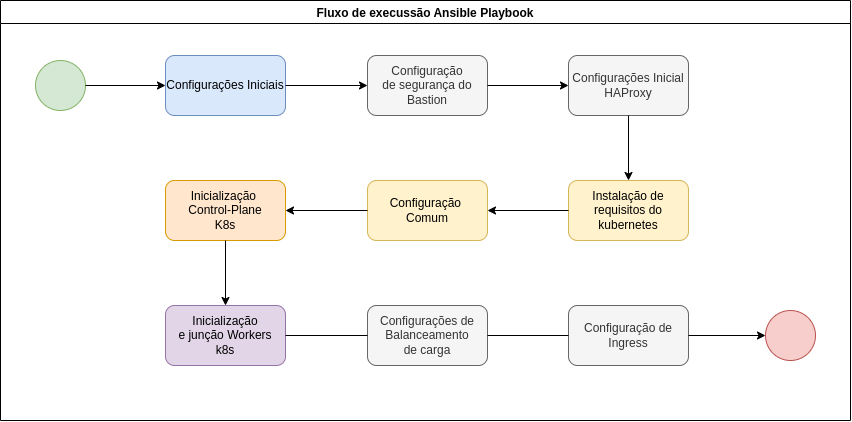
\includegraphics[width=\linewidth]{04-figuras/ansibleflow.png}
    \caption{Fluxo de Execussão do Ansible Playbook}
    \label{fig:ansibleflow}
\end{figure}

A formulação do inventário considera que os computadores a serem confiugrados estejam na mesma rede do bastion, sendo que toda a configuração passa por ele, garantindo assim a segurança da execussão apenas para outros computaodres que possam ser estabelicdas conexão a partir dele. Esse inventário também divide em grupos as maquinas, podendo assim ser executado o playbook novamente para novas maquinas a serem adicinadas a \emph{cluster}  que garante o recrutamento estático de novos nós para comporem o cluster, e virtualmete podendo chegar no limite de rede no qual os nós d \emph{cluster} stão agrupado sob. Para garantir a correta execussão o invetário pode ser referenciado explicitamente durante a execussão desde que tenha o mesmo formato do disponibilizado no repositório.

\subsection{Configurações de infra do cluster}
O provisionamento de novas cargas de trabalhos e \emph{stacks} de processamento de dados foram realizados utilizando terraform\textregistered \ que garantiu a correta gestão do estado recursos provisionados n \emph{cluster} m junção do helm\textregistered \ como ferramenta de \emph{deploy} de aplicações. Essa combinação garantiu a máxima eficiência, gerenciando as dependencias entre recursos e aplicações durante tempo de execussão e garantindo a imutabilidade dos recursos provisionados, o que diminui o \emph{drift} ou desvio de configurações, minimizando anti padrões como \emph{snowflake}\cite{snowflakeanti}

\subsection{Gestão de armazenamento no cluster}
StorageClass é a forma mais recomendada para gerenciamento de CSI (\emph{container storage interface}) de disponiblizar volumes compartilhados n \emph{cluster} e Kubernetes\textregistered, porém em \emph{clusters }\emph{bare-metal} e não existem muitas opções de \emph{provider} CSI que não necessitem de um software ou ainda hardware específico, como SANs (\emph{StorageAreaNetwork}) específícos. Sem CSI, as chamadas de \emph{filesystem} que são executados pelos containers que alocam PVC (\emph{persistent volumes claim}) podem incorrer em erros o que gera perda de dados ou ainda erros de IO. 


Tendo como premissa que alguns volumes devem estar disponiveis para o cluster, e não ao container, não é possivel utilizar PV (persistent volumes) ou StorageClasses que sejam locais, ou sejam que não disponibilizem aquele volume a \emph{cluster} omo um todo, uma vez que um pod ao ser encerrado por qualquer motivo pode ser alocado novamente em outro nó do cluster, que não possuirá qualquer registro da informação escrita anterioremente. 

Com isso resumimos a duas alternativas abertas: Ceph e NFS. Ambos os protocolos possuem CSI. Primeiramente optou-se por utilizar o Ceph, uma vez que esse protocolo possibilitaria o uso de toda a capacidade de armazenamento d \emph{cluster} e forma compartilhada, e com isso somaria-se os volumes disponiveis localmente, podendo resultar em um volume elástico que aumentaria toda vez que um nó fosse adicionado ao cluster, somando a capacidade de armazenamento d \emph{cluster} omo um todo. 

Após algumas tentativas de implementação, o funcionamento correto e esperado do driver não foi alcançado. E mesmo sendo a opção mais indicada, tendo um grau de complexidade que estrapolou o tempo disponivel foi substituído pelo driver NFS, que garante a disponibilidade de volumes compartilhados, mas é baseado apenas no volume local do servidor que o provê. Mesmo tendo menos benefícios, ainda atende o proposito de volumes compartilhados, e pode ser usado em uma estratégia \emph{mesh}, que garantiria uma soma de volumes entre os nós do cluster, mas que precisaria ser adaptado para ser disponiblizado como um pool de storageclasses, também fugindo do intento desse trabalho.

Por fim visando a possivel subistituição do servidor NFS, por um NAS (\emph{Netware Area Storage}) que é uma solução de hardware específico ou generico (configurável) e portanto sendo mais viável do ponto de vista econômico (preço/volume). Vale ressaltar que o menor custo vem com problemas de latência, o que pode prejudicar o desempenho de soluções de processamnto de dados que sejam intensivos em leitura e escrita de dados, especialmente o segundo.

Para tornar a solução viável em termos de complexidade de configuração, disponiblidade de hardware e custo, optou-se por usar o servidor bastion e \emph{load balancer} como também servidor de NFS. Como o numero de requisições realizadas n \emph{cluster} inda não será tão grande, uma vez que a maior parte das requisições serão internas e de coomandos, não foi mapeado como um risco de desempenho, mas tornando o uso mais intenso do cluster, seria recomendado isolar a função de server de NFS para um NAS ou servidor específico.

\section{Disponibilização das imagens de container}

Diversas dependencias para a execussão das tarefas e logo apos a exploração visual e analise dos dados coletados pela orquestração devem ser incorporada as imagens base utilizadas para o Airflow e também Jupyter. Para controlar a entrega dessas imagens e disponibiliza-las para o servidor, foi publicado em um repositório de imagens publica, com credenciais que expiravam em 12horas. Essas imagens utilizaram uma estratégia tag para \emph{release} associada ao \emph{commit message} no repositório do git, podendo assim recuperar versões específicas e rastrear mudanças que possivelmente alteraram o comportamento esperado dos containers que as utilizarem. 

Essa tag era então substituida por meio de variaveis no terraform e assim utilizadas para configuração dos recursos durante o tempo de deploy das aplicações com as novas tags. Essa estratégia garante um fluxo auditavel de mudanças e preconiza a imutabilidade uma premissa para uso de infraestrutura como código. 

\section{Orquestração do processamento}
A configuração do processo de ETL para ingestão dos dados do banco de medicamentos industrializados foi organizado de acordo com a figura \ref{fig:airflowdag}.
\begin{figure}[!ht]
    \centering
    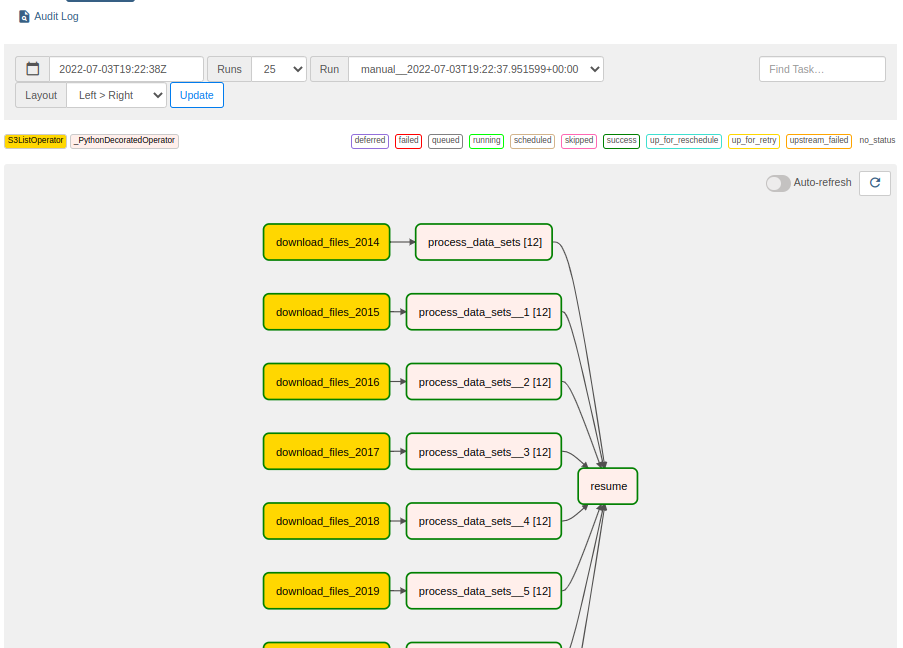
\includegraphics[width=0.8\linewidth]{04-figuras/graph_execution.png}
    \caption{ETL DAG}
    \label{fig:airflowdag}
\end{figure}

Apesar de não representado há uma etapa precessora, um \emph{operator} que lista os anos disponiveis para criação de grupos de \emph{mapper} de tarefas dinâmicas, é um \emph{fan-out} de duas etapas, lançando os arquivos que irão listar anos disponvieis em bucket S3 na AWS, outro que listará os arquivos disponiveis de cada ano, e seu download.

Na etapa de processamento seguinte carrega os dados desses arquivos em memória, em um \emph{dataframe} do {pandas} (biblioteca python). Pelo tamanho dos arquivos, não é possivel fazer o carregamento de uma só vez e por tanto a opção de chunks foi usado, isso particiona os dados para garantir o processo por partes. Essa opção garante que diversas tarefas sejam executadas em parelelo sem sobrecarregar  \emph{cluster} em mesmmo causar eventos de OOM (\emph{out of memory}) causando assim que a tarefa entre na fila de \emph{retry}.

O ponto de configuração dos containers foi de 1vCPU e 2GB de RAM para processar arquivos entre 0.5-0.7GB de dados por vez, como a tabela de escrita dos dados processado no PostgreSQL era a mesma para para garantir a consolidação dos dados, o pipeline de execussão de cada tarefa ficava entre entre 4 e 12 minutos desde o momento de início do \emph{download} até o completo carregamento em banco. Como a operação de escrita em banco também é uma atividade restrita, ou seja, não permite duas escritas simultaneas, esse com certeza era um ponto de restrição do fluxo de dados. A possivel solução para esse gargalo era a escrita dos dados pre-processados em tabelas distintas e em um passo seguinte a consolidação em tabela única. Porém para manter a estrutura de um ETL simples e validar o processamento no cluster, não foi necessário realizar essas etapas de otimização. 

Mencionado as limitações ja observadas, é necssário indicar mais uma importante restrição que o banco também esta sendo executado n \emph{cluster} om 1,5GB de RAM e 0.3 vCPU, sendo um recurso compartilhado entre diversos outros recursos d \emph{cluster} or ter mais de um banco na mesma instância. E ainda utilizando CSI de NFS, que como mencionado anteriormente adiciona latência e conhecidamente não performa muito bem em usos intensos de escritas.

\begin{figure}[!ht]
    \centering
    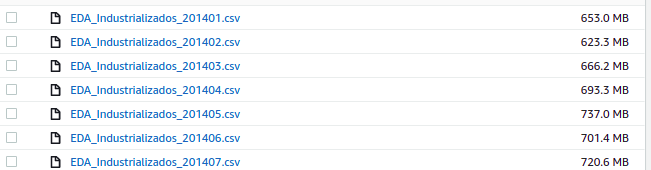
\includegraphics[width=0.8\linewidth]{04-figuras/s3_size.png}
    \caption{S3 armazenamento dos dados}
    \label{fig:s3_storage}
\end{figure}


Considerando o tamanho e tempo de execussão das atividades podemos inferir que:
\begin{itemize}
    \item o tempo de execussão total dessas tarefas de forma serial, seria de aproximadamente $8 min\ *\ 90 arquivos = 96min$ para importar todos os arquivos
    \item mesmo com as execussões simultaneas limitadas a 12, não utilizamos 50\% do cluster
\end{itemize} . 


\begin{figure}[!ht]
    \centering
    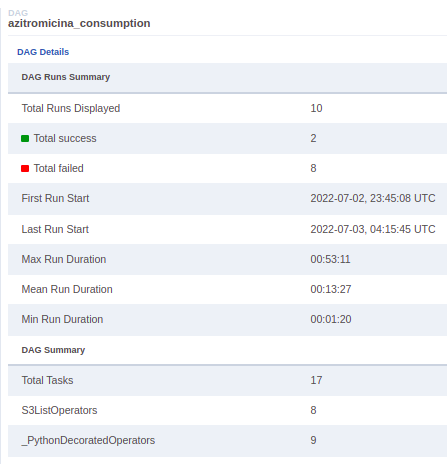
\includegraphics[width=0.5\linewidth]{04-figuras/report_execution_summary1.png}
    \caption{Relatório de execussão}
    \label{fig:report}
\end{figure}

É possivel avaliar que a sobreposição de tarefas é gerenciada pelo airflow mantendo a restrição de 12 execussões por vez na figura \ref{fig:gantt},

\begin{figure}[!ht]
    \centering
    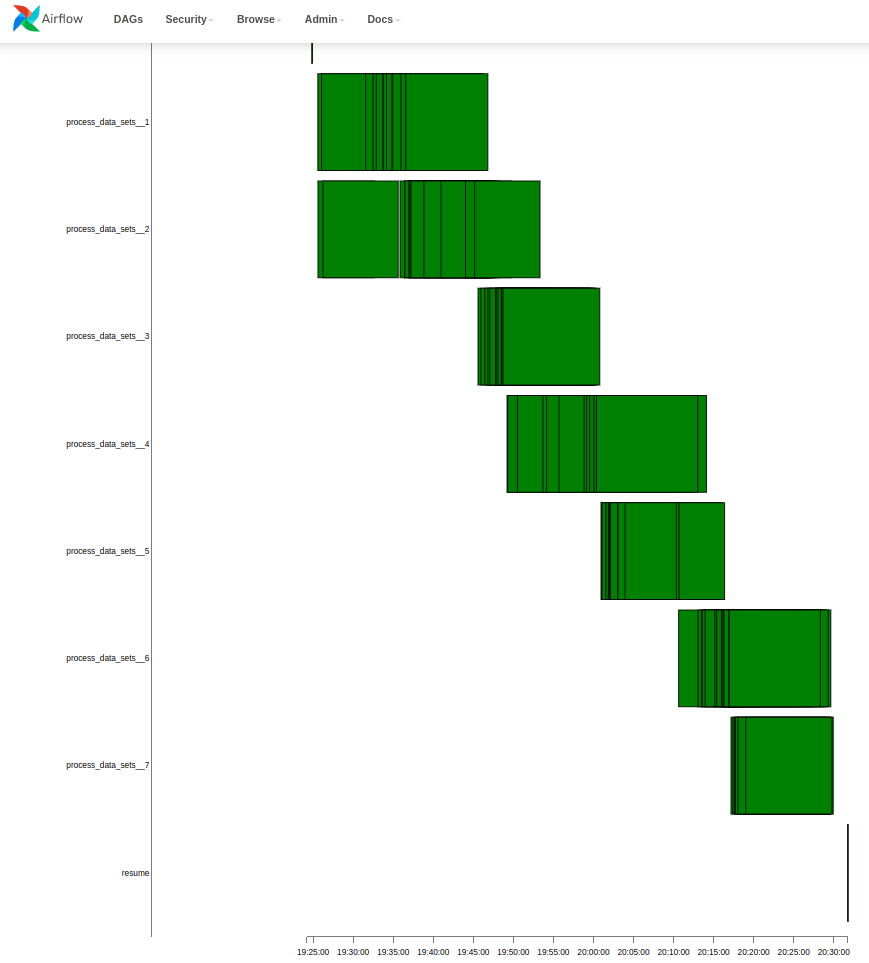
\includegraphics[width=0.7\linewidth]{04-figuras/gantt.png}
    \caption{Grafico de Gantt da orquestração}
    \label{fig:gantt}
\end{figure}

Porém o tempo total gasto foi de 53 min, segundo a figura \ref{fig:report}. O que representa 55\% do tempo esperado. Mesmo considerando as restrições de desempenho citadas anteriormente.

Pode se inferir que o numero de execussões simultaneas representavam 24vCPUs e 48GB de memória por limite de tarefas em execussão, representando um servidor que sozinho custaria entre 20 e 40 mil reais, e nesse trabalho utilizou maquinas que não estavam sendo utilizadas do DCC UFMG.



\section{Analise de dados}
Todas as análises foram executas em um jypter notebooks provisionado no cluster.

Um total de 95.345.640 prescrições de azitromicina foram atendidas em farmácias e drogarias do Brasil, entre 2015 e 2021. A maioria dos pacientes para os quais foi dispensado o medicamento era do sexo feminino (53,62\%), com média de idade de 32,75 (± 2,04). Entre as regiões com maior venda de azitromicina destacam-se as regiões Sudeste (47,44\%) e Sul (22,47\%) e entre as UF, destacam-se São Paulo (24,76\%), Minas Gerais (13,17\%) e Rio Grande do Sul (12,49\%) Tabela \ref{table:base_desc}

\begin{table}[!htbp]
    \centering
    \begin{tabular}{llll}
    \hline
    \multicolumn{2}{l}{\multirow{2}{*}{\textbf{Características}}} & \textbf{n} & \textbf{\%} \\ \cline{3-4} 
    \multicolumn{2}{l}{}                                          & 95345640   & 100         \\ \hline
    \multicolumn{2}{l}{\textbf{Sexo do paciente}}                 &            &             \\
                         & Feminino                               & 50051932   & 53,62       \\
                         & Masculino                              & 45293708   & 46,38       \\
    \multicolumn{2}{l}{\textbf{Região}}                           &            &             \\
                         & Centro Oeste                           & 8325772    & 8,73        \\
                         & Nordeste                               & 15311389   & 15,44       \\
                         & Norte                                  & 5050278    & 5,3         \\
                         & Sudeste                                & 45232822   & 47,44       \\
                         & Sul                                    & 21425379   & 22,47       \\
    \multicolumn{2}{l}{\textbf{Unidade Federativa}}               &            &             \\
                         & Acre                                   & 235293     & 0,25        \\
                         & Alagoas                                & 587010     & 0,62        \\
                         & Amapá                                  & 251408     & 0,26        \\
                         & Amazonas                               & 541218     & 0,57        \\
                         & Bahia                                  & 3672405    & 3,85        \\
                         & Ceara                                  & 2545617    & 2,67        \\
                         & Distrito Federal                       & 1205841    & 1,26        \\
                         & Espírito Santos                        & 1704011    & 1,79        \\
                         & Goiás                                  & 5007864    & 5,25        \\
                         & Maranhão                               & 1414456    & 1,48        \\
                         & Mato Grosso                            & 1068418    & 1,12        \\
                         & Mato Grosso do Sul                     & 1043649    & 1,09        \\
                         & Minas Gerais                           & 12552967   & 13,17       \\
                         & Pará                                   & 2640661    & 2,77        \\
                         & Paraíba                                & 2207241    & 2,31        \\
                         & Paraná                                 & 5818312    & 6,1         \\
                         & Pernambuco                             & 1823847    & 1,91        \\
                         & Piauí                                  & 861105     & 0,9         \\
                         & Rio de Janeiro                         & 7372345    & 7,73        \\
                         & Rio Grande do Norte                    & 1653179    & 1,73        \\
                         & Rio Grande do Sul                      & 11911733   & 12,49       \\
                         & Rondônia                               & 693489     & 0,73        \\
                         & Roraima                                & 199669     & 0,21        \\
                         & Santa Catarina                         & 3695334    & 3,88        \\
                         & São Paulo                              & 23603499   & 24,76       \\
                         & Sergipe                                & 546529     & 0,57        \\
                         & Tocantins                              & 488540     & 0,51        \\ \hline
    \end{tabular}
    \caption{Características das prescrições de azitromicina atendidas em farmácias e drogarias, Brasil, 2014-2020.}
    \label{table:base_desc}
    \end{table}

    No período de 6 anos, em números absolutos, o número de prescrições de azitromicina, no Brasil, aumentou de 13.421.249 prescrições em 2014 para 17.735.901 prescrições em 2020, representando um aumento de 32,1\%. Considerando o crescimento da população, isso representa um aumento na taxa de prescrição de azitromicina de 66,2 para 83,8 prescrições por 1.000 habitantes, em todo o período Tabela \ref{table:base_region}. 


    \begin{table}[!htbp]
        \centering
    \begin{tabular}{llrr}
    \hline
    \multicolumn{2}{l}{\multirow{2}{*}{\textbf{Localidade}}} & \multicolumn{2}{l}{\textbf{Taxa prescrição / $10^4$ hab}} \\ \cline{3-4} 

    \multicolumn{2}{l}{}                                     & \textbf{2014}              & \textbf{2020}              \\ \hline
    \multicolumn{2}{l}{\textbf{Brasil}}                      & 66,2                       & 83,8                       \\
    \multicolumn{2}{l}{\textbf{Unidade Federativa}}          &                            &                            \\
                      & Acre                                 & 30,2                       & 71,9                       \\
                      & Alagoas                              & 20,5                       & 42,8                       \\
                      & Amapá                                & 36,5                       & 79,2                       \\
                      & Amazonas                             & 13                         & 38                         \\
                      & Bahia                                & 46,3                       & 51,5                       \\
                      & Ceara                                & 23,8                       & 38,3                       \\
                      & Distrito Federal                     & 52,7                       & 96,9                       \\
                      & Espírito Santos                      & 49,6                       & 97,8                       \\
                      & Goiás                                & 133,2                      & 116,1                      \\
                      & Maranhão                             & 19,6                       & 31,1                       \\
                      & Mato Grosso                          & 31,3                       & 73,5                       \\
                      & Mato Grosso do Sul                   & 49,4                       & 79,2                       \\
                      & Minas Gerais                         & 66,2                       & 149,2                      \\
                      & Pará                                 & 30,6                       & 49,4                       \\
                      & Paraíba                              & 145,2                      & 101,7                      \\
                      & Paraná                               & 57,8                       & 129,2                      \\
                      & Pernambuco                           & 26,2                       & 39,3                       \\
                      & Piauí                                & 116,8                      & 33,7                       \\
                      & Rio de Janeiro                       & 44,1                       & 76,2                       \\
                      & Rio Grande do Norte                  & 50                         & 106,7                      \\
                      & Rio Grande do Sul                    & 137,6                      & 97,4                       \\
                      & Rondônia                             & 37,5                       & 109,4                      \\
                      & Roraima                              & 37,3                       & 99,8                       \\
                      & Santa Catarina                       & 61,3                       & 84,5                       \\
                      & São Paulo                            & 96,6                       & 86,7                       \\
                      & Sergipe                              & 30,7                       & 58,6                       \\
                      & Tocantins                            & 34,5                       & 80,6                       \\ \hline
    \end{tabular}
    \caption{Taxas de prescrição de azitromicina atendidas em farmácias e drogarias, no Brasil, em 2014 e 2020}
    \label{table:base_region}
    \end{table}

    A maioria das UF apresentaram aumento nas taxas de prescrição de azitromicina por 1.000 habitantes, com destaque para: Minas Gerais (66,2 para 149,2 prescrições por 1.000 habitantes), Rondônia (37,5 para 109,4 prescrições por 1.000 habitantes) e Roraima (37,2 para 99,8 prescrições por 1.000 habitantes).
Considerando apenas os anos de 2019 e 2020, como períodos pré e durante a pandemia da COVID-19, respectivamente, observa-se que houve aumento nas taxas de prescrição no Brasil e em todas UF, exceto no Rio de Janeiro (87,3 para 76,2 prescrições por 1.000 habitantes) e no Rio Grande do Sul (106,6 para 97,4 prescrições por 1.000 habitantes) (Tabela \ref{table:base_region1}).
\begin{table}[!htbp]
    \centering
\begin{tabular}{llrr}
    \hline
    \multicolumn{2}{l}{\multirow{2}{*}{\textbf{Localidade}}} & \multicolumn{2}{l}{\textbf{Taxa prescrição / $10^4$ hab}} \\ \cline{3-4} 
    \multicolumn{2}{l}{}                                     & \textbf{2019}              & \textbf{2020}              \\ \hline
    \multicolumn{2}{l}{\textbf{Brasil}}                      & 59,9                       & 83,8                       \\
    \multicolumn{2}{l}{\textbf{Unidade Federativa}}          &                            &                            \\
                      & Acre                                 & 32,3                       & 71,9                       \\
                      & Alagoas                              & 23,5                       & 42,8                       \\
                      & Amapá                                & 45,9                       & 79,2                       \\
                      & Amazonas                             & 17,3                       & 38                         \\
                      & Bahia                                & 31,9                       & 51,5                       \\
                      & Ceara                                & 29,7                       & 38,3                       \\
                      & Distrito Federal                     & 57,3                       & 96,9                       \\
                      & Espírito Santos                      & 62,5                       & 97,8                       \\
                      & Goiás                                & 74,3                       & 116,1                      \\
                      & Maranhão                             & 18,5                       & 31,1                       \\
                      & Mato Grosso                          & 49,2                       & 73,5                       \\
                      & Mato Grosso do Sul                   & 56,4                       & 79,2                       \\
                      & Minas Gerais                         & 81,7                       & 149,2                      \\
                      & Pará                                 & 27,3                       & 49,4                       \\
                      & Paraíba                              & 62,3                       & 101,7                      \\
                      & Paraná                               & 66,3                       & 129,2                      \\
                      & Pernambuco                           & 27,2                       & 39,3                       \\
                      & Piauí                                & 22,1                       & 33,7                       \\
                      & Rio de Janeiro                       & 87,3                       & 76,2                       \\
                      & Rio Grande do Norte                  & 73                         & 106,7                      \\
                      & Rio Grande do Sul                    & 106,6                      & 97,4                       \\
                      & Rondônia                             & 58,8                       & 109,4                      \\
                      & Roraima                              & 38,9                       & 99,8                       \\
                      & Santa Catarina                       & 73,3                       & 84,5                       \\
                      & São Paulo                            & 68,1                       & 86,7                       \\
                      & Sergipe                              & 36                         & 58,6                       \\
                      & Tocantins                            & 44,1                       & 80,6                       \\ \hline
    \end{tabular}
    \caption{Taxas de prescrição de azitromicina atendidas em farmácias e drogarias, no Brasil, em 2019 e 2020}
    \label{table:base_region1}
    \end{table}

    Os maiores aumentos nas taxas de prescrição de azitromicina foram observados em Minas Gerais (81,7 para 149,2 prescrições por 1.000 habitantes), Paraná (66,3 para 129,2 prescrições por 1.000 habitantes), Roraima (38,9 para 99,8 prescrições por 1.000 habitantes), Rondônia (58,8 para 109,4 prescrições por 1.000 habitantes) e Goiás (74,3 para 116,1 prescrições por 1.000 habitantes). 

    Pode se observar os numero absolutos na figura \ref{fig:presc_ano_estadp}


    Pode-se observar que o resultado é coerente quando avaliado sob a perspectiva do Tau de Kendal como descrito na figura \ref{fig:tau}, que avalia correção de crescimento entre variáveis. Os estados do Amazonas, Mato Grosso, Mato Grosso do Sul, Paraná, Pará, Rio grande do Norte, Santa Catarina e Tocantins, apresentam um alto grau de correlação de crescimento no tempo e com significância estatistica (P < 0.05). Apesar dos resultados para o estado de Minas Gerais descrito acima, o mesmo não apresenta uma significância estatistica adequada, o que pode ser causdo pelo aumento populacional do estado, o que pode mascarar o aumento da taxa de prescrição.
    \begin{figure}[!ht]
        \centering
        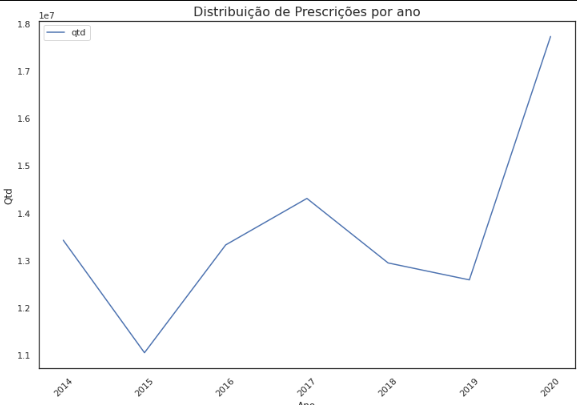
\includegraphics[width=0.8\linewidth]{04-figuras/distribuicao_presc_ano.png}
        \caption{Precrição por ano}
        \label{fig:presc_ano}
    \end{figure}
    \begin{figure}[!ht]
        \centering
        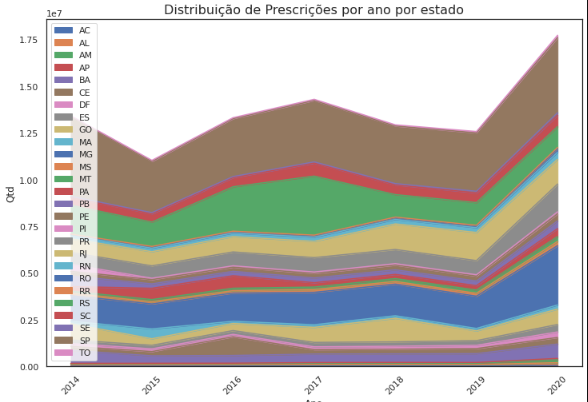
\includegraphics[width=0.8\linewidth]{04-figuras/distribuicao_presc_ano_estado.png}
        \caption{Precrição por ano por estado}
        \label{fig:presc_ano_estadp}
    \end{figure}
    \begin{figure}[!ht]
        \centering
        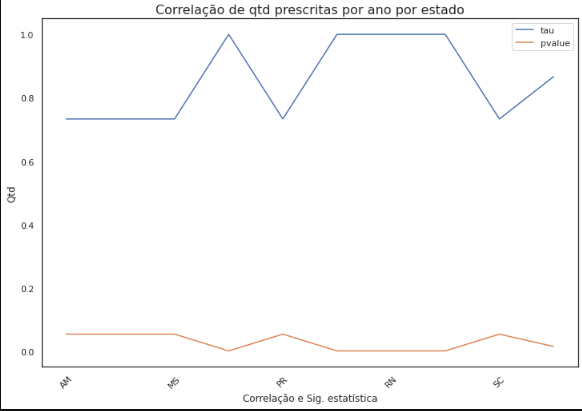
\includegraphics[width=0.8\linewidth]{04-figuras/corelaticao_estados.png}
        \caption{Precrição por ano}
        \label{fig:tau}
    \end{figure}

    Pode se ainda traçar um paralelo entre os dados dispostos até o momento e a inclinação politica dos estados. Sendo o governo o maior promotor e divulgador do kit COVID, que continnha azitromicina como um medicamento anti-bacteriano para combate ao vírus do COVID-19.  Estados mais afetados como os da região norte, assim como regiões como centro-oeste que são regiões majoritariamente eleitoras do governo promotor da kit COVID e portanto apresentam também maior adoção e maior correlação de crescimento das prescrições de azitromicina no periodo da COVID-19.

    \begin{figure}[!ht]
        \centering
        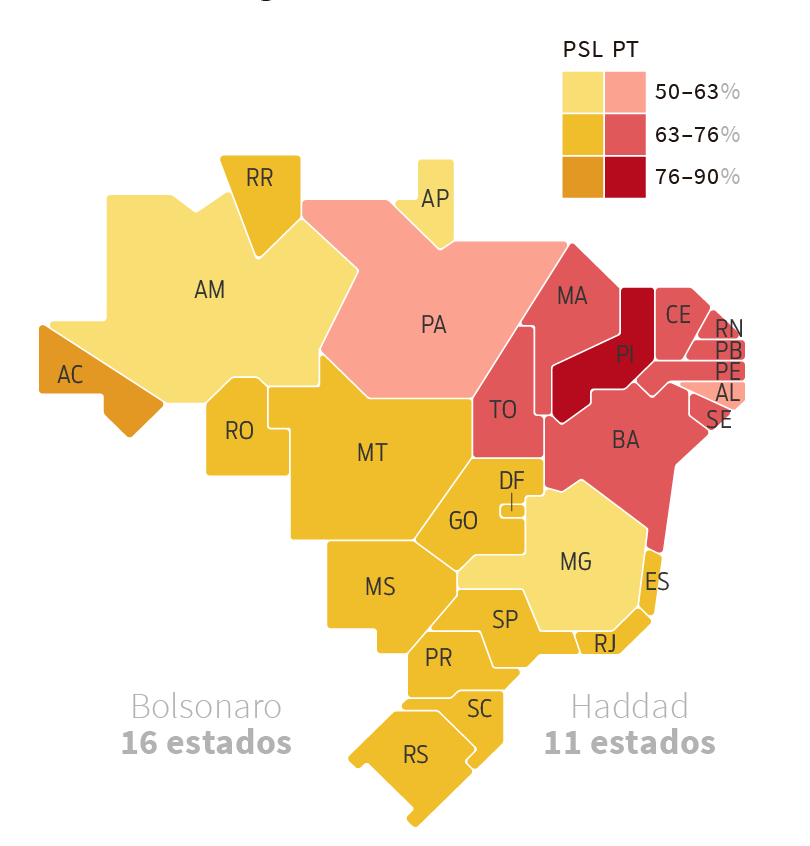
\includegraphics[width=0.8\linewidth]{04-figuras/estados_eleitores_atual_governo.png}
        \caption[Divulgação do resultado da eleição presidencial de 2018]{Divulgação do resultado da eleição presidencial de 2018 (Fonte: Gazeta do Povo, 2018) }
        \label{fig:tau}
    \end{figure}